\documentclass[tikz]{standalone}
\usepackage{pgfplots}
\pgfplotsset{compat=1.15}
\usepackage{mathrsfs}
\usetikzlibrary{arrows,calc}
\usepackage{tkz-euclide}

\pagestyle{empty}

\definecolor{AngleClr}{rgb}{0,0.39215686274509803,0}
\definecolor{ShapeClr}{rgb}{0.6,0.2,0}

\begin{document}

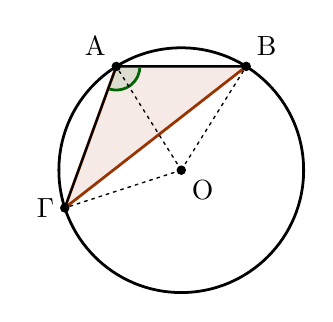
\begin{tikzpicture}[scale=.75]
\tkzSetUpLine[line width=1pt,color=black]
\tkzSetUpPoint[fill=black]

\tkzDefPoints{0/0/B,2.2/0/C}

\tkzDefPoint(-110:2.55){A}

\tkzDefTriangleCenter[circum](A,B,C) \tkzGetPoint{O}
\tkzDrawCircle[black,line width=1.0pt](O,A)

\tkzFillPolygon[fill=ShapeClr,fill opacity=0.1](A,B,C)

\tkzFillAngle[fill=AngleClr,size=.4,fill opacity=0.1](A,B,C)
\tkzMarkAngle[line width=1pt,size=.4,color=AngleClr](A,B,C)

\tkzDrawPolygon[color=ShapeClr](A,B,C)

\tkzDrawSegments[line width=0.5pt,color=black,dashed,dash pattern=on 1pt off 1.75pt](O,A O,B O,C)

\tkzDrawPoints[size=3](A,B,C,O)
\tkzLabelPoint[left](A){$\rm \Gamma$}
\tkzLabelPoint[above left](B){$\rm A$}
\tkzLabelPoint[above right](C){$\rm B$}
\tkzLabelPoint[below right](O){$\rm O$}

\tkzDrawSegments[line width=0.75pt](A,B B,C)

\end{tikzpicture}

\end{document}
